\chapter{Introducción}
\begin{figure}[h]
\centering
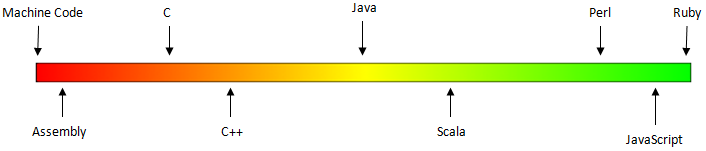
\includegraphics[scale=0.5]{Niveles}
\captionsetup{justification=centering}
\caption[caption]{\footnotesize Niveles de Programación en el Computador. \\ \textbf{Fuente:} \texttt{http://www.codecommit.com/blog/java/defining-high-mid-and-low-level-languages}}
\end{figure}